\documentclass[•]{article}
\usepackage{huy}

\begin{document}
\section{Entity-Relationship Modeling\cite{connolly2005database}}
ER modeling is an approach to database design that begins by identifying the important data
called entities and relationships between the data that must be represented in
the model. \par 
Some basic concepts of ER model:
\begin{description}
\item[Entity type.] A group of objects with the same properties, which are identified by the enterprise as having an independent existence.
\item[Relationship type.] A set of meaningful associations among entity types.
\item[Attribute.] A property of an entity or a relationship type.
\item[Primary key.] The candidate key that is selected to uniquely identify each occurence of an entity type.
\end{description}
\section{Relationships Between Entities \cite{beal} }
There are three types of relationships between entities:
\begin{description}
\item[One-to-one]One instance of an entity (A) is associated with one other instance of another entity (B). For example, in a database of employees, each employee name (A) is associated with only one social security number (B).
\item[One-to-many]One instance of an entity (A) is associated with zero, one or many instances of another entity (B), but for one instance of entity B there is only one instance of entity A. For example, for a company with all employees working in one building, the building name (A) is associated with many different employees (B), but those employees all share the same singular association with entity A.
\item[Many-to-many]One instance of an entity (A) is associated with one, zero or many instances of another entity (B), and one instance of entity B is associated with one, zero or many instances of entity A. For example, for a company in which all of its employees work on multiple projects, each instance of an employee (A) is associated with many instances of a project (B), and at the same time, each instance of a project (B) has multiple employees (A) associated with it.
\end{description}
\section{Practical part}
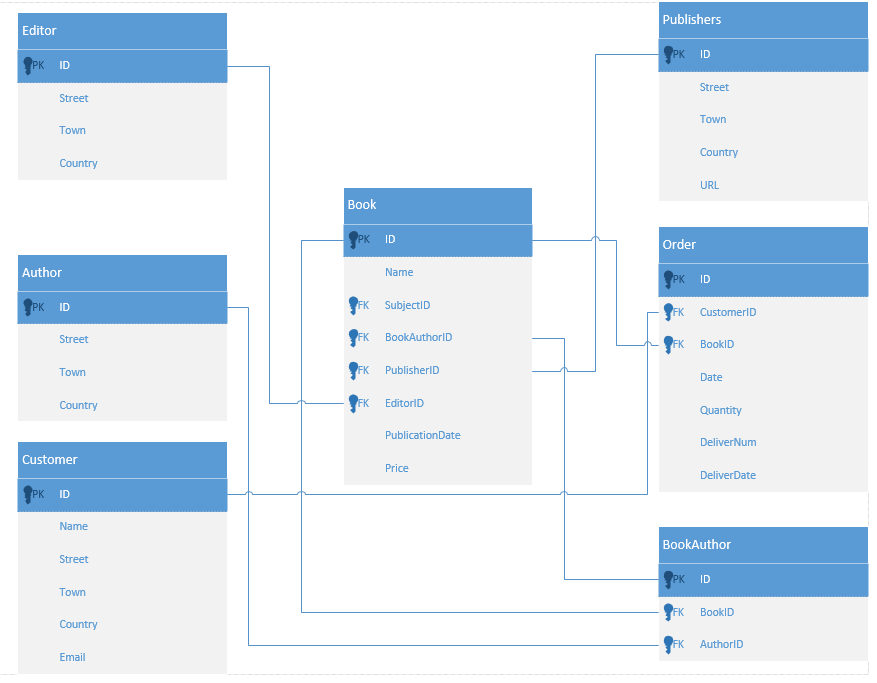
\includegraphics[width=\textwidth]{UML-model.PNG}
\bibliographystyle{plain}
\bibliography{references}
\end{document}